\chapter[Conclusions and Outlook]{Conclusions and Outlook}

In this body of work we present three methods of resonator development that focus on manipulating the magnetic field profile in order to improve the sensitivity of EPR spectroscopy of proteins. These efforts span from 9.5 to 420~GHz.  

The introduction of the uniform field re-entrant TE$_{\text{01U}}$ resonator at Q-band (35~GHz) in Chapter~3 improves EPR sensitivity by providing true $\pi/2$ and $\pi$ pulses. This has an advantage in pulse experiments with complex sequences used to manipulating the spin system. For example, HYSCORE data at Q-band will benefit from uniform magnetic field excitation by providing a cleaner mixing pulse which will maximize the nuclear transition mixing and remove on-diagonal signals. \cite{Doorslaer2007,Harmer2009} Such signals typically dominate the spectrum and make interpretation difficult. For EDNMR, a uniform magnetic field excitation translates into a reduction of the width of the central peak allowing for the measurement of modulation frequencies typically dominated by this feature. \cite{NicholasCox2013} Finally, the increase in resonator bandwidth allows the spectroscopist to utilize the state-of-the-art arbitrary waveform generators for further signal improvement and method development. \cite{DOLL201327,dSegawa2015,SPINDLER201730,WILI201826,PRISNER201998}

In Chapter~4, the experiments in the THz-bandgap with meta-materials made from an array of split-ring resonators at 420~GHz serve as an interesting example of using analytical lumped-circuit transmission-line theory to fully reproduce the EPR signal of the split-ring resonator coupled to a spin. The use of split-ring resonators create a cross-sectional area that is not limited by the wavelength of the operating frequency. The split-ring resonators maintain an active depth proportional to the individual geometry providing a suitable volume for thin film samples. An EPR signal enhancement is measured at the operating frequency of the split-ring resonators. With the new understanding outlined in this work, it may be possible to design for a series of multi-frequency high-field EPR experiments with meta-material resonant discs at each frequency. This will allow spectroscopists to probe the zero-field splitting characteristics of high-spin samples in thin films.

The introduction of the self-resonance micro-helix at X-band (9.5~GHz) in Chapter~5 provides a resonator efficiency of 3.2~mT/W$^{1/2}$ corresponding to a $\pi/2$ pulse of 20~ns with an incident power of 20~mW. The self-resonant micro-helix exhibits an absolute sensitivity increase up to a factor of 28 in EPR signal improvement compared to commercial resonators. For samples that saturate readily, such as protein samples, the micro-helix provides a factor of 6 in absolute EPR sensitivity improvement compared to commercial resonators. This translates into a factor of 36 in measurement time for equivalent sample volumes. Additionally, the high resonator efficiency and low $Q_0$-value (bandwidth of 90~MHz critically coupled) provides an opportunity to measure FID induced EPR on systems without costly high-powered amplifiers, further extending the usefulness of pulse EPR spectroscopy.

Finally, the self-resonant micro-helix provides an advance in resonator design that has allowed, for the first time, the collection of EPR data from a 0.3 $\times$ 0.1 $\times$ 0.1~mm$^3$ single crystal of [FeFe]-hydrogenase in the H$_{ox}$ state from {\em Clostridium pasteurianum} (CpI) at a temperature of 15~K. Full $g$-tensor analysis been successfully performed and a proposed orientation of the principal axes is discussed. With the excellent signal-to-noise ratio, data was collected using an ESEEM/HYSCORE pulse sequence. These data show an angle dependant $^{14}$N hyperfine- and quadrupole-tensor originating from either the cyanide-ligand of the distal iron or the ADT-ligand.  To our knowledge, the ESEEM/HYSCORE spectra collected herein are the first published results from a protein single-crystal with a volume less than 27~nL at X-band. Although initial ESEEM data has been obtained, a finer angular resolution is needed to follow the modulation frequencies. Analysis and assignment of these modulate frequencies from the interaction with the active-site co-factor is to follow. 

\begin{figure*}[htbp]
\centering
 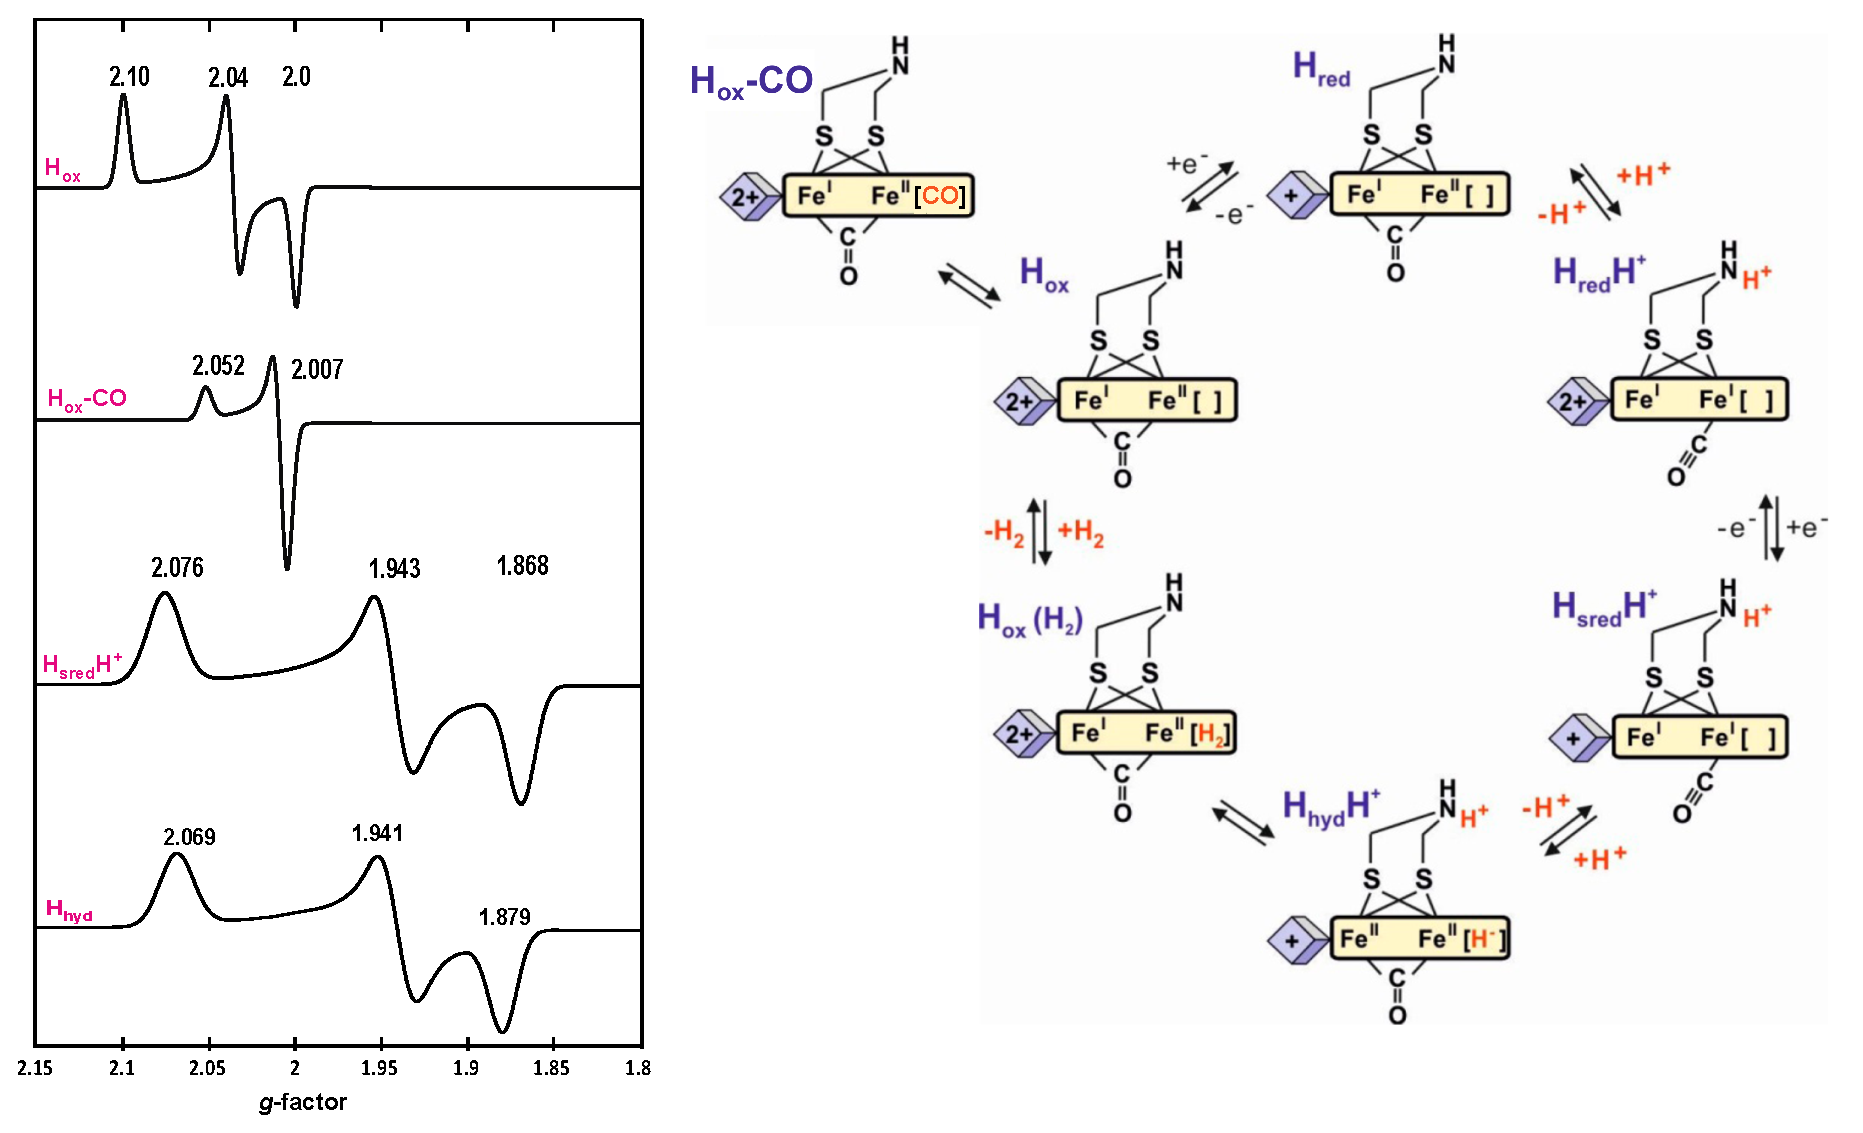
\includegraphics[width=\textwidth]{Kapitel/end-images/Ch6-EPRCat.eps}
 \caption[EPR Signals along the catalytic cycle of FeFe-Hydrogenase.]{Shown are simulations of the EPR signal from paramagnetic intermediates of frozen solution samples along the catalytic cycle of [FeFe]-hydrogenase is displayed on the left. A simplified catalytic cycle showing the redox states of the distal and proximal iron and [4Fe4S] clusters is displayed on the right.} 
 \label{fig:FeFeCatCycle}
\end{figure*}

Focusing on [FeFe]-hydrogenase, further studies of g-tensor and hyperfine-tensor interactions are now feasible in single-crystal experiments. Shown in Fig.~\ref{fig:FeFeCatCycle} are the simulations of the frozen solution spectra relating to the intermediates on the proposed catalytic cycle. \cite{lubitzhyd} Crystals of suitable size (0.8-3 nL) are available of the [FeFe]-hydrogenase CpI in the H$_{ox}$ state, studied herein, and a reduced CpI-apo which has an EPR signal derived from the reduced four [4Fe4S]$^+$ clusters. In CpI-apo, the H-cluster is not present. The CPI-apo crystal could be used to study the electron transfer pathway of the [FeFe]-hydrogenase and how it relates to the function of the hydrogenase at various redox potentials. It is also possible to obtain crystals in the inactive H$_{ox}$-CO state, which may lend insight into reducing the oxygen sensitivity of the [FeFe]-hydrogenase. Such studies will further protein engineering and artificial enzyme research for creating bio-inspired and bio-mimicking hydrogenase systems. \cite{C7SE00582B}


{\renewcommand{\bibsection}{\clearpage\section*{\bibname}\markboth{\bibname}{\bibname}}
\renewcommand{\bibname}{REFERENCES}
\bibliographystyle{elsarticle-num}
\bibliography{Kapitel/Ch5-References}
}